\newcounter{counter}
\newcommand\DiffTitle{%
  \frametitle{\refstepcounter{counter} Diffusion/Heat equation~\thecounter}}
\resetcounteronoverlays{counter}


\begin{frame}[fragile]
\DiffTitle
\begin{itemize}
\item Diffusion equation or heat equation.
      \begin{fleqn}
      \begin{equation}
      \frac{\partial T}{\partial t} = \kappa \frac{\partial^2 T}{\partial x^2}
      \label{eq:heat}
      \end{equation}
      \end{fleqn}

\item The boundary condition
\begin{fleqn}
      \begin{equation}
       T\left(x,0\right) = \begin{cases} f\left(x\right) \qquad Neumann \ BC \\ 
      const. \qquad Dirichlet \ BC \end{cases} \qquad \forall x \in \left[0,L\right]
      \end{equation}
      \end{fleqn}      
      
\end{itemize}
\end{frame}

\begin{frame}[fragile]
\DiffTitle
\begin{itemize}
\item Diffusion/Heat equation in one-dimension
\begin{figure}
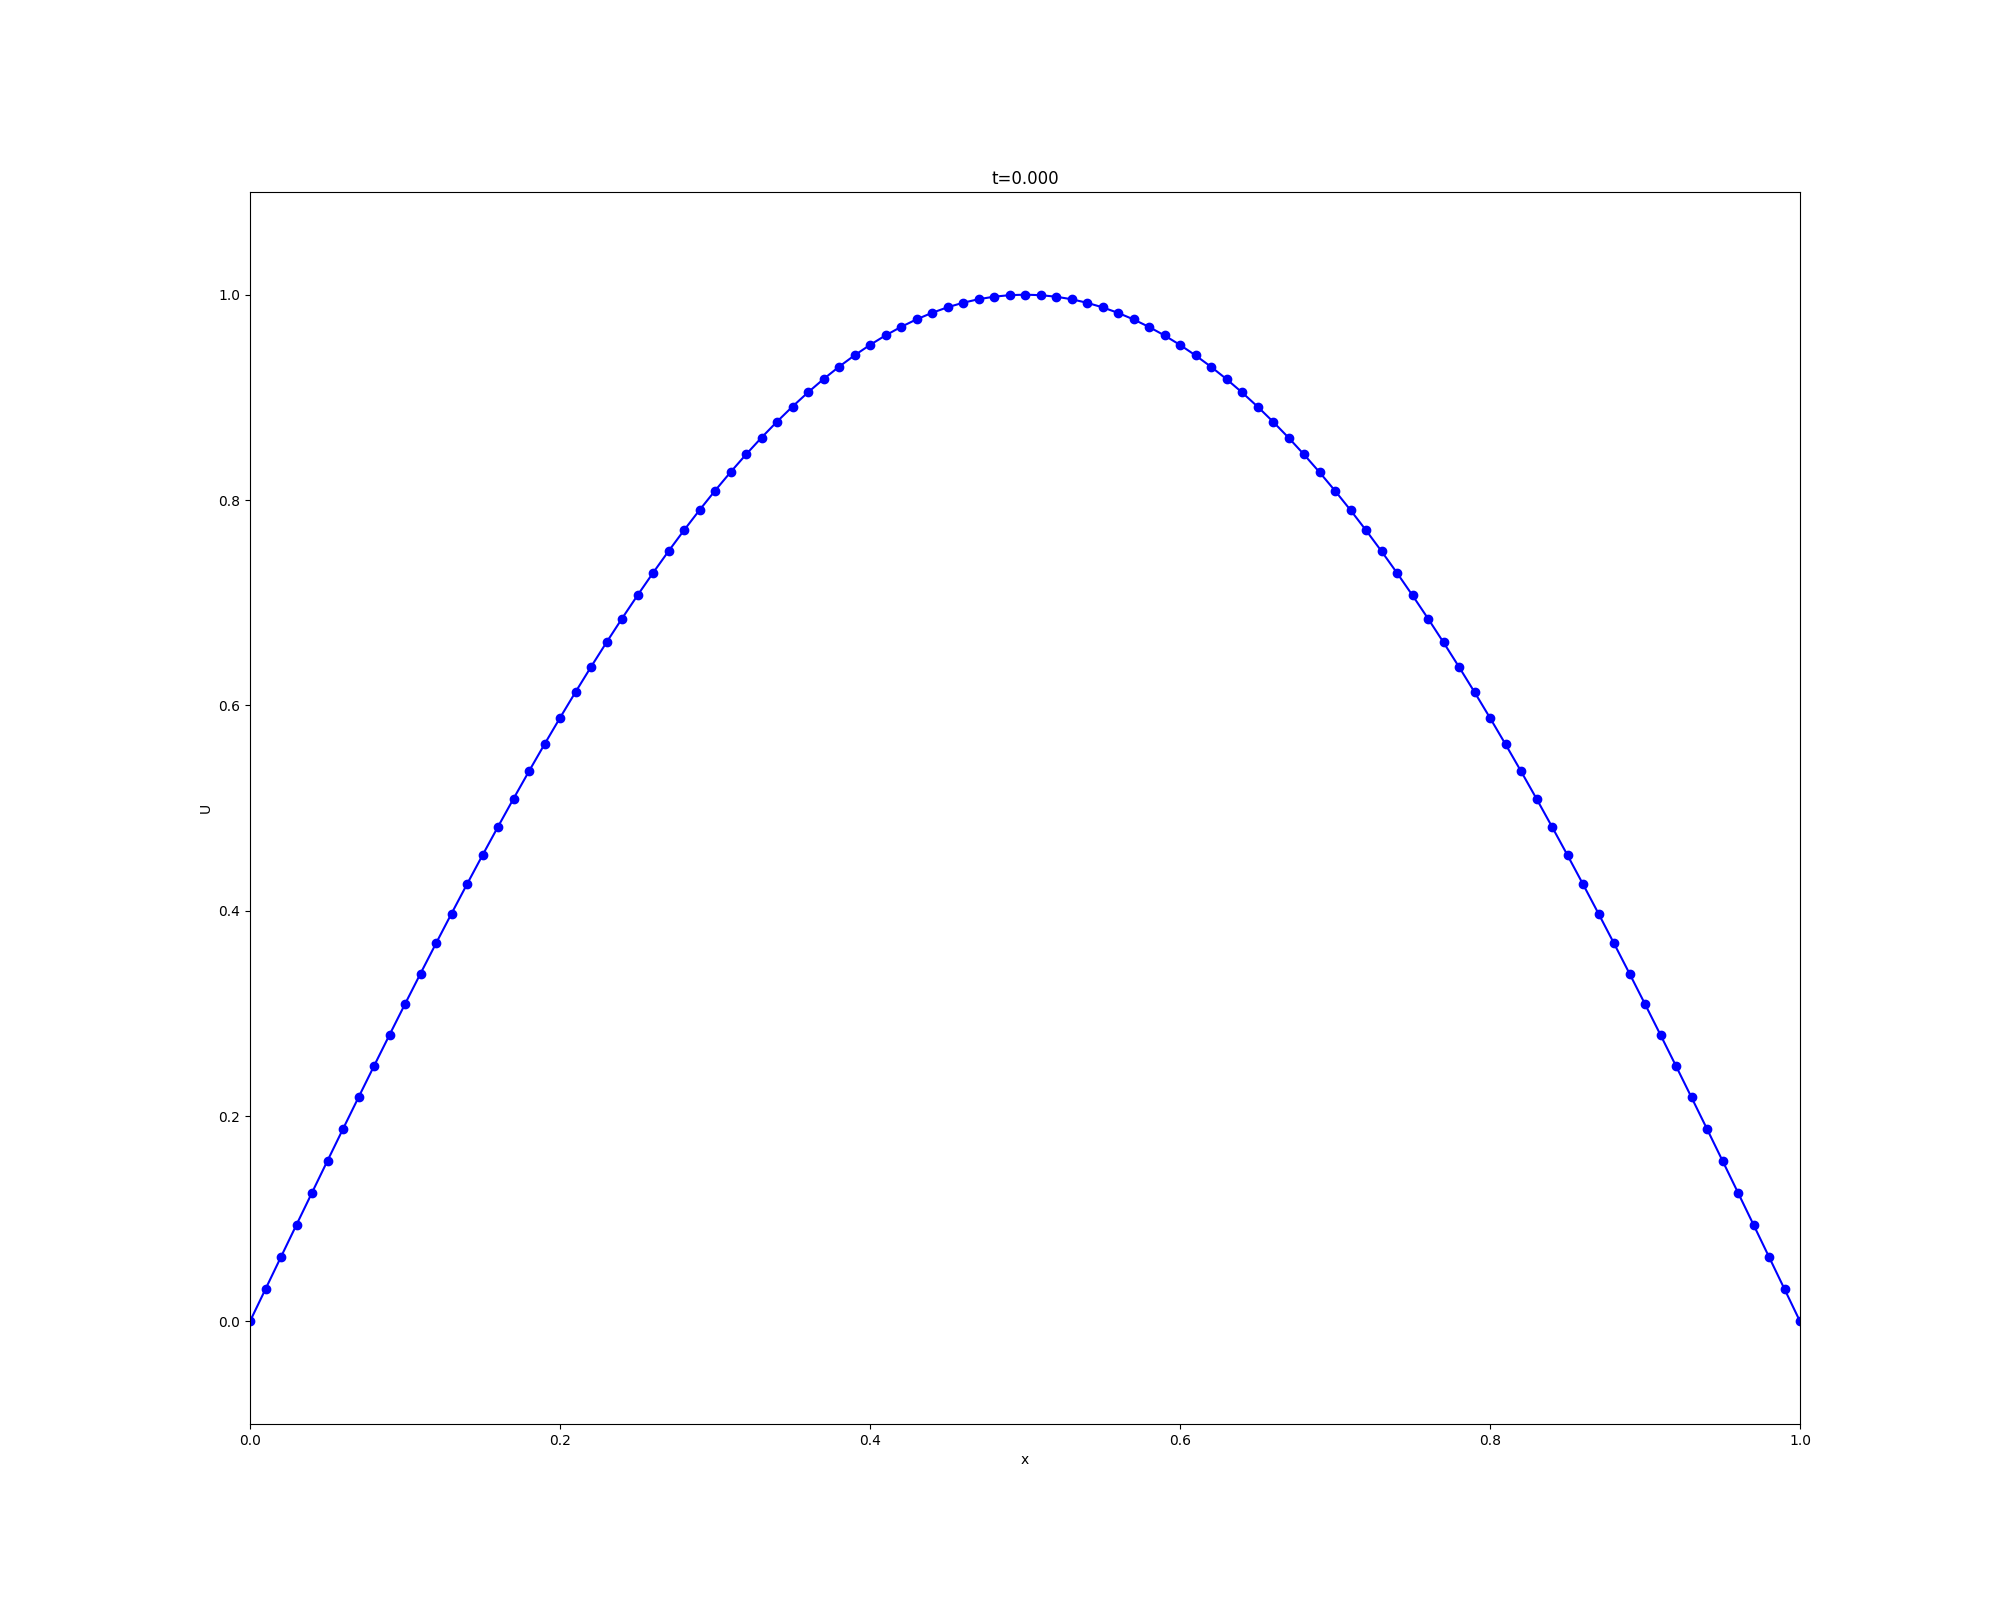
\includegraphics[width=0.5\textwidth, height=0.25\textwidth]{./image/diff_init.png}%
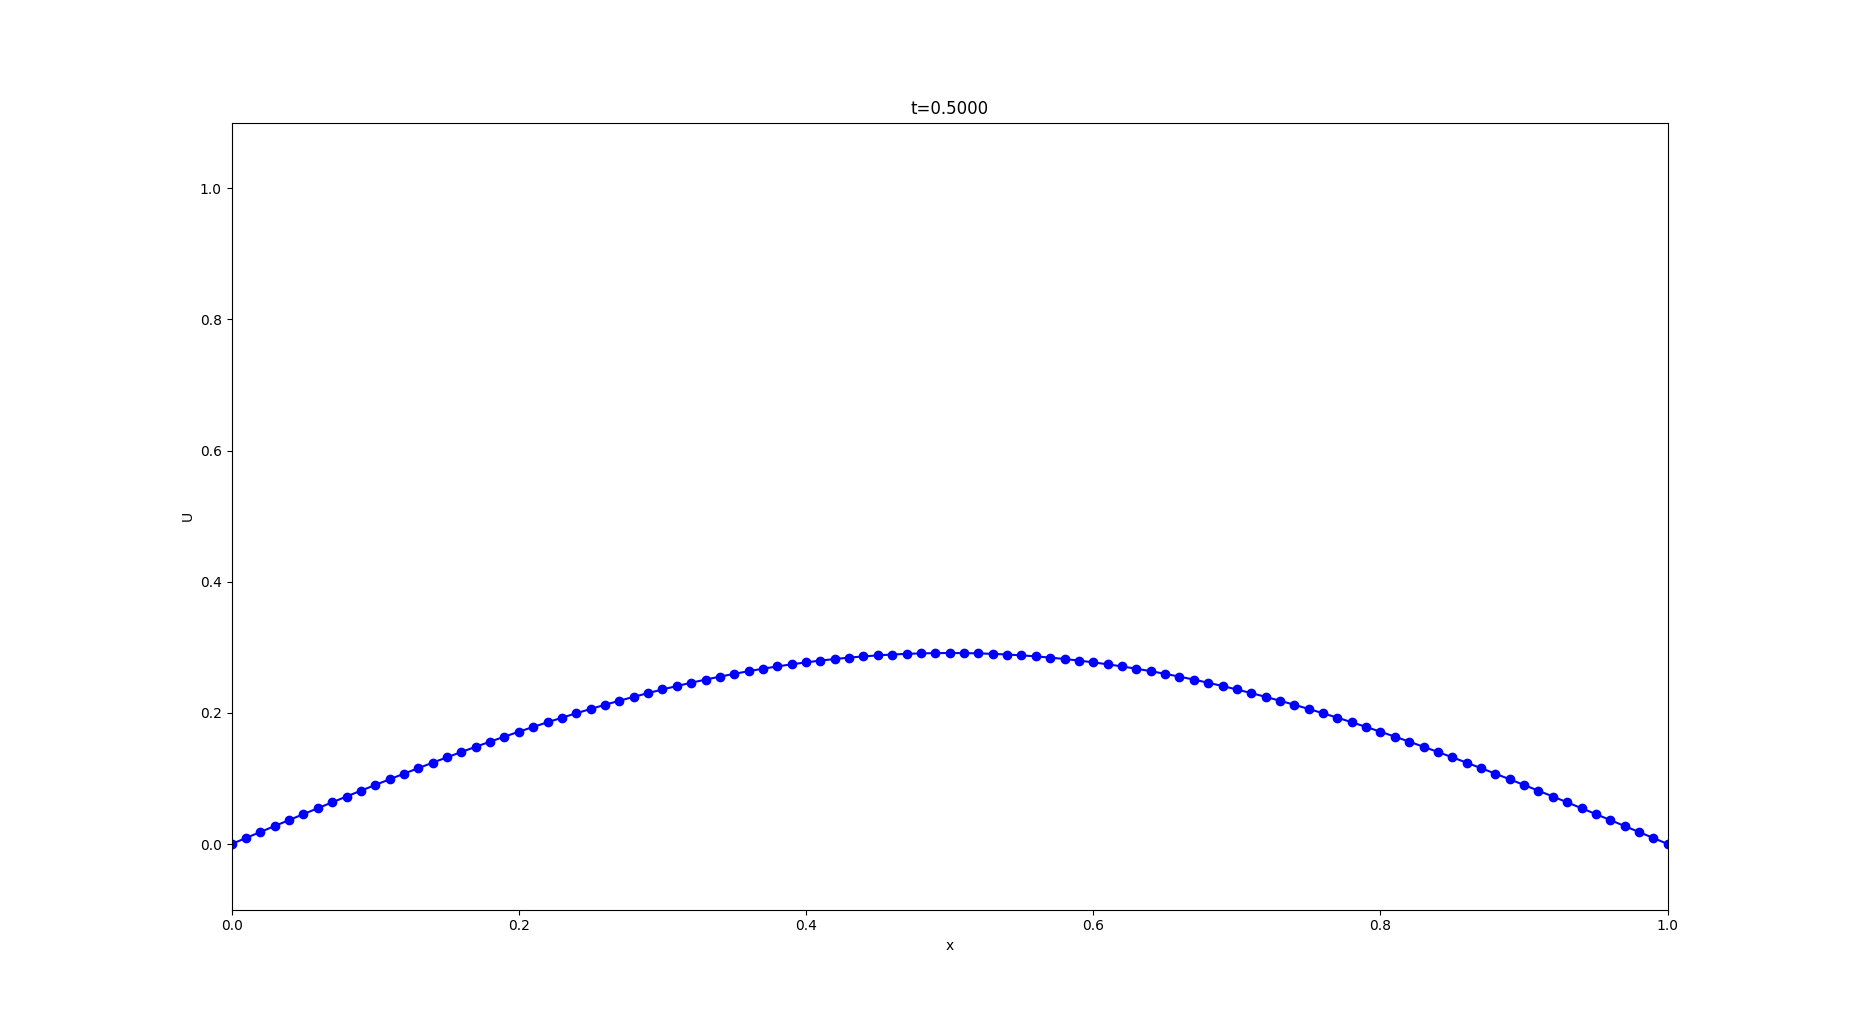
\includegraphics[width=0.5\textwidth, height=0.25\textwidth]{./image/diff_final.png}
\caption{Left is at t=0.0000 and right is at t=0.5000}
\end{figure}
\end{itemize}
\end{frame}

\begin{frame}[fragile]
\DiffTitle
\begin{itemize}
\item Sample of the heat equation discretization in Python.
\lstinputlisting[language=Python, firstline=47, lastline=57]{./codes/heat1D.py}
\end{itemize}
\end{frame}